\documentclass{article}

\usepackage[english]{babel}
\usepackage[utf8]{inputenc}

\usepackage[inline,shortlabels]{enumitem}
\usepackage{amsmath, amssymb}
\usepackage{xcolor, ifthen}
\usepackage{siunitx} % represent numbers with separators
\usepackage{csquotes}
\usepackage{graphicx, multirow}
\usepackage{subcaption}
\usepackage{accents} % provides \accentset, used in Problem Formalization.


\usepackage{tikz, pgfplots}
%\usetikzlibrary{ fit, calc, arrows, shapes }

% from http://tex.stackexchange.com/questions/157389/how-to-center-column-values-in-a-table
\usepackage{array}
\newcolumntype{P}[1]{>{\centering\arraybackslash}p{#1}}

\newcommand{\red}[1]{{\color{red} #1}}
\newcommand{\green}[1]{{\color{green} #1}}
\newcommand{\yellow}[1]{{\color{yellow} #1}}

\def\todo{\red{TODO}}



\newcommand{\multibinom}[2]{
  \left(\!\middle(\genfrac{}{}{0pt}{}{#1}{#2}\middle)\!\right)
}

% \newcommand{\crule}[2][1][1px]{
%   \begin{center} \rule{#1\textwidth}{#2} \end{center}
% }

\begin{document}

\begin{abstract}
  \todo
\end{abstract}

\bigskip
\tableofcontents
\newpage


\section{Introduction}

Classes scheduling is a \emph{constraints satisfaction problem} (CSP).
and all scheduling problems share a common constraint: schedule consistency ---
one cannot participate in several events at the same time. For the classes case,
the participants are:
\begin{enumerate*}
  \item \emph{groups} of students,
  \item teachers or \emph{professors},
  \item \emph{classrooms}.
\end{enumerate*}
The first two are represented by real people and the rooms are represented by
the institution.

Problem \emph{constraints} can be divided into:
\begin{enumerate}
  \item \underline{Class constraints}: a class should be a productive event, so
    a professor should be able to \emph{teach} the class, the classroom should
    have the \emph{capacity} to hold all the students and be properly \emph{equipped},
    and the group should be \emph{inscribed} to class subject
    (further called \emph{discipline}).
  \item \underline{Time constraints}: no participant can have two classes
    at the same time (or intersecting in time), as mentioned before.
  \item \underline{Strong restrictions}: the restrictions, put on a participant, that
    \emph{must} be respected. May include working hours, fixed lunch recess time,
    and any other institution or person specific \emph{obligations}.
  \item \underline{Weak restrictions}: the restrictions, that \emph{should} be respected,
    but are not critical to the solution. Compliance with theese restrictions
    raises \emph{solution quality}, but it is assumed that the all of them
    cannot be fully met for all the participants --- they are intended to
    represent personal \emph{preferences}.
\end{enumerate}

The goal is finding a solution --- schedule, satisfying all the constraints.
University schedule is composed of \emph{individual schedules} for every
participant. An individual schedules may be seen as a day-time table with
classes in the cells. Therefore the complete schedule can be represented as a
3-dimentional table, as shown in figure \ref{fig:ScheduleSpace}.
\bigskip

\begin{figure}
  \label{fig:ScheduleSpace}
  
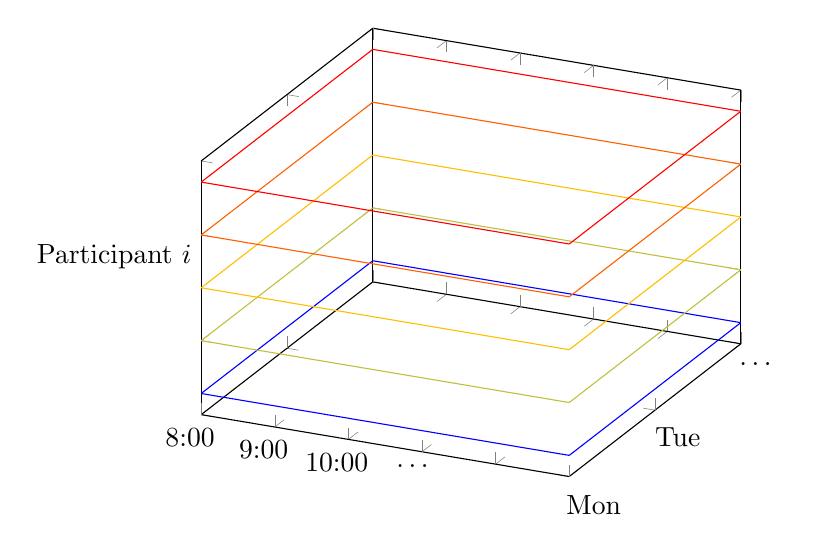
\begin{tikzpicture}

\begin{axis}[
  xlabel=, % Time,
  xticklabels={, 8:00, 9:00, 10:00, $\dots$},
  ylabel=, %Day,
  yticklabels={, Mon, Tue, $\dots$},
  zlabel=, %Participant,
  zticklabels = {, , ,Participant $i$}
  ]

  \foreach \i in {1,...,5}
     \addplot3[surf] coordinates { (0,0,\i) (1,0,\i) (1,1,\i) (0,1,\i) (0,0,\i)  };

  % \addplot3[surf] coordinates { (0,0,0) (1,0,0) (1,1,0) (0,1,0) (0,0,0)  };
  % \addplot3[surf] coordinates { (0,0,1) (1,0,1) (1,1,1) (0,1,1) (0,0,1)  };

\end{axis}


\end{tikzpicture}

  \caption{University schedule is a 3-dimentional table. Horizontal rectangles
           represent invividual schedules for the corresponding participants.
          }
\end{figure}


Scheduling problems are \emph{n-p complete} \cite{ULLMAN1975384}
and therefore the optimal solution can be found within finite (polynomial) time.
But being finite, doesn't make the required time acceptable.
To ensure solution perfection, one must consider \emph{every possible} classes
configuration.

For example, six working days in a week and twelve time slots every day
(every hour from 8:00 to 20:00), would yield $6 \times 12 = 72$ options
to place each class.
Given that each group needs five diferent disciplines to be asssigned,
there would be  $\multibinom{72}{5} = 18474840$ possible classes assignment for
each group (without considering professors and classrooms).
Thus, the time, required to find the \emph{optimal solution}, might exceed any
reasonable limits, if the university is big.

This problem is a typical one for the CSPs, and many researchers have
been looking for means of solving such problems within reasonable time.
During the last years different algorithms and techniques where developed,
such as
\emph{dynamic constraint satisfaction based on extension particle swarm
      optimization algorithm} \cite{CSPswarm},
\emph{dynamic state bounding} \cite{CSPdynStateBound},
\emph{conflict-vector detection} \cite{CSPtimetable},
\emph{neural networks} \cite{CSPneuro},
\emph{ant colony optimization} \cite{CSPcunningACO, CSPlimmemACO},
\emph{selective hyper-heuristics} \cite{CSPhypHeur}
and \emph{agents} \cite{CSPagent2013, CSPagent2014, DCSPagent1998}.


The \emph{agent negotiation} approach is usually used for solving distributed
CSPs (DCSPs) \cite{DCSPagent1998, DCSP2013, CSPagent2014}.
In this case the constrains are \emph{distributed} among the agents instead of
being gathered in one place.

\red{Such constraints distribution is useful for the \emph{classes scheduling} problem
, because it permits to distribute not only the constraints, but also the solution. }
Each agent would be expected to \emph{negotiate} a suitable solution for its
``master'', without concerning itself with the schedules of the others.
Tthe combined solution can be obtained as soon as all the participants agree on
their timetables.

\documentclass[ThesisDoc]{subfiles}
\begin{document}


\green{Explicar que son los CSP}
\section{Constraint Satisfaction Problems}

\green{Poner una definición no formal}
\medskip

There are many problems that require positioning or assigning something,
respecting established \emph{restrictions}. \emph{Graph coloring} and
\emph{n-queen} chess problem are classical constraint satisfaction problems (CSPs).

\medskip
\green{Poner algunos ejemplos}
\medskip

The graph coloring problem comes from cartography, where it was needed to color
countries on political maps, in such a way that no country had a land border with
a country of the same color. It was found that \textbf{any} map can be colored
with only four colors.

The n-queen problem is known in chess as \emph{eight queen puzzle}.
Queens in chess can move/attack to/at any square,
that is in a the same row, column or diagonal with the queen.
In the puzzle one needs to place eight (the size of a chess desk)
queens on the desk, so that none of them is threatened by another.
N-queens problems is a generalization of that puzzle, where $n$ queens need
to be placed on a $n \times n$ desk.

Constraint satisfaction problems are found in many areas:
machine vision, natural language processing, theorem proving,
planning and in our problem --- scheduling \cite{MAS}.


\subsection{Formal definition}
%%%%%%%%%%%%%%%%%%%%%%%%%%%%%%%%%%%%%%%%%%%%%%%%%%%%%%%%%%%%%%%%%%%%%%%%%%%%%%%%
\noindent
Formally speaking, a CSP is defined by its \emph{variables} $V$ with the
corresponding \emph{domains} and the \emph{constraints} $\{\xi\}$
over values assignation \cite{MAS}.

\begin{align*}
  V                &= \{v_i\}_{i=1}^N
& \{{\dot v}^i_j\} &= \domain(v_i)
& \xi              &: \{{\dot v}^i_\ast\}_{i=1}^N \mapsto [0,1]
\end{align*}


A variable defines a ``slot'' that can hold a value from the corresponding domain.
A solution to CSP is an assignation of the values ${\dot v}^i_\ast$
to the variables $V$, such that all the restriction hold.
\begin{equation}
  {\dot V} = \{{\dot v}^i_\ast\}_{i=1}^N \text{is a solution}
   \iff \forall \xi \in \{\xi\} \Rightarrow \xi({\dot V}) = 1
\end{equation}

The constraints above are defined in the most generalized form,
over the entire solution. There is a particular case, that is found in many problems
--- \emph{binary constraints}, imposed on \emph{pairs} of values:
$$\xi_2 : \left< {\dot v}^i_\ast, {\dot v}^j_\ast \right> \mapsto \{0,1\}$$

If all constrains are binary, than the satisfaction condition is
$$\forall \xi_2     \in \{\xi\},~
  \forall v_i, v_j  \in V | v_i \not= v_j
~ \Rightarrow ~ \xi_2(v_i, v_j) = 1
$$

\medskip

In the graph coloring problem, the variables are the \emph{colors to be assigned}
for each graph node $\{n_i\}_{i=1}^N$. In this case, all the variables have
the same domain values: four colors, for example \textit{Red}, \textit{Green},
\textit{Blue} and \textit{Yellow}. The constraint is binary and depends on graph
structure:
$$ \xi_2(x,y)= \begin{cases}
  0 & \mbox{if } \exists \text{~edge~} x \leftrightarrow y
                ~\land \text{~color~} x = \text{color~} y \\
  1 & \text{otherwise}
\end{cases}
$$

% For the n-queens problem, there are two ways of representing the variables.One
% can see queens' positions as a single variable --- pairs $\left< x,y \right>$.
% But it's better to handle them separately, as it would be shown in \ref{TODO}.
% In this case each queen would have two variables:
% horizontal and vertical positions $x$ and $y$.

For the n-queens problem, the variables are queens' positions ---
pairs $\left< x,y \right>$, where $x$ is queen's horizontal position and
$y$ is the vertical one. The restrictions can be gathered within a single
constraint function:
$$\xi_2(\left<x_1,y_1\right>, \left<x_2,y_2\right>) =
    \begin{cases}
      0 & \mbox{if } \begin{cases}
                        &      x_1 = x_2  \lor y_1 = y_2 \\
                        \lor~& x_1 = y_2 \land x_2 = y_1 \\
                        \lor~& |x_1-y_1| = |x_2-y_2|
                     \end{cases} \\
     1 & \text{otherwise}
    \end{cases}
$$

\todo\red{: needs to be rewritten after the introduction is done}

  In our \emph{university classes scheduling} problem (UCSP) the variables
are personal schedules, called \emph{timetables} in this thesis,
for each \emph{participant}: professor and group/student.
  A timetable consists of the day-time slots, where classes can be put.
  A \emph{class} is formed for teaching a group a specific \emph{subject},
connecting the participants (of each kind) and establishing a classroom and
the beginning--end \emph{time}.
  Problem \emph{constraints} can be divided into:
\begin{enumerate}
  \item \underline{Class constraints}: a class should be a productive event, so
    a professor should be able to \emph{teach} the class, the classroom should
    have the \emph{capacity} to hold all the students and be properly \emph{equipped},
    and the group should be \emph{inscribed} to class subject
    (further called \emph{discipline}).
  \item \underline{Time constraints}: no participant can have two classes
    at the same time (or intersecting in time), as mentioned before.
  \item \underline{Strong restrictions}: the restrictions, put on a participant, that
    \emph{must} be respected. May include working hours, fixed lunch recess time,
    and any other institution or person specific \emph{obligations}.
  % \item \red{\underline{Weak restrictions} (MOVE)}: the restrictions, that \emph{should} be respected,
  %   but are not critical to the solution. Compliance with these restrictions
  %   raises \emph{solution quality}, but it is assumed that the all of them
  %   cannot be fully met for all the participants --- they are intended to
  %   represent personal \emph{preferences}.
\end{enumerate}

\bigskip

%%%%%%%%%%%%%%%%%%%%%%%%%%%%%%%%%%%%%%%%%%%%%%%%%%%%%%%%%%%%%%%%%%%%%%%%%%%%%%%%
  Until now we were speaking about restrictions satisfactions, but the problem can
be extended to an \emph{optimization} one by defining an
\emph{objective function} over the values configurations.

  Unlike the restrictions (that yield boolean result), the objective functions
should have continuous codomains:
$$\tilde\xi : \{{\dot v}^i_\ast\}_{i=1}^N \mapsto \Re$$
  In order to facilitate the calculations and erase the internal differences of
the objectives, it's often required that the functions must be normalized:
the co-domains are restricted to $[-1,1]$ or $[0,1]$ intervals.

  For example, in case of our UCSP,
one can add \underline{personal preferences} or some institution criteria as
optimization parameters.
  Compliance with the preferences raises \emph{solution quality},
but it is assumed that the all of them cannot be fully met for all the
participants, because \emph{personal} preferences are often
contradictory for different persons.

\subsection{Solution Methods}
%%%%%%%%%%%%%%%%%%%%%%%%%%%%%%%%%%%%%%%%%%%%%%%%%%%%%%%%%%%%%%%%%%%%%%%%%%%%%%%%
\green{Explicar por qué son importantes computacionalmente}\\
\medskip

\noindent
  Solving these problems usually presents difficulties due to the amount of
possible combinations to consider for a solution. Let's have a look at
some university schedule.
  For example, six working days in a week and twelve time slots every day
(every hour from 8:00 to 20:00), would yield $6 \times 12 = 72$ options
to place each class.
  Given that each group needs, for example, five different disciplines to be assigned,
there would be  $\multibinom{72}{5} = \num[group-separator={,}]{18474840}$
possible classes assignments for each group,
even without considering professors and classrooms.

\bigskip
%%%%%%%%%%%%%%%%%%%%%%%%%%%%%%%%%%%%%%%%%%%%%%%%%%%%%%%%%%%%%%%%%%%%%%%%%%%%%%%%
\green{Explicar formas de resolver los CSP} \todo
\medskip
\noindent

  The researchers have been looking for means of solving such
problems within reasonable time.
  During the last years different algorithms and techniques where developed,
such as
\emph{dynamic constraint satisfaction based on extension particle swarm
      optimization algorithm} \cite{CSPswarm},
\emph{dynamic state bounding} \cite{CSPdynStateBound},
\emph{conflict-vector detection} \cite{CSPtimetable},
\emph{neural networks} \cite{CSPneuro},
\emph{ant colony optimization} \cite{CSPcunningACO, CSPlimmemACO},
\emph{selective hyper-heuristics} \cite{CSPhypHeur}
and \emph{agents} \cite{CSPagent2013, CSPagent2014, DCSPagent1998}.

\medskip

Those methods do not seek for the optimal solutions, focusing instead on
``rather good'' ones, that can be obtained within reasonable time using admissible
computing resources.

\bigskip

\todo \red{: write something about one of the techniques}



\subsection{Distributed problems}
%%%%%%%%%%%%%%%%%%%%%%%%%%%%%%%%%%%%%%%%%%%%%%%%%%%%%%%%%%%%%%%%%%%%%%%%%%%%%%%%
Agents approach allows solving CSPs in a distributed manner, also distributing
the problem knowledge and constraints
\cite{DCSPagent1998, DCSP2013, CSPagent2014, MAS, MAS-Survey}.

\begin{displayquote}[\cite{MAS-Survey}] % \cite[p.~2]{MAS-Survey}
  For example, a constraint satisfaction problem can often be
  decomposed into several not entirely independent
  subproblems that can be solved on different processors. $\dots$
  MAS (Multiagent System) allows the sub-problems of a constraint satisfaction
  problem to be subcontracted to different problem solving agents with their own
  interests and goals.
\end{displayquote}

\noindent
Such problems are \emph{Distributed Constraints Satisfaction Problems} (DCSPs).
\begin{displayquote}[\cite{MAS}] % \cite[p.~4]{MAS}
  In a distributed CSP, each variable is owned by a different agent. The goal is
  still to find a global variable assignment that meets the constraints, but each agent
  decides on the value of his own variable with relative autonomy. While he does
  not have a global view, each agent can communicate with his neighbors in the
  constraint graph.
\end{displayquote}

  The constrains are distributed alongside the variables: an agent knows only the
constrains over the variable it owns. A DCSP can also have objective functions for
optimization.

  The UCSP fits perfectly into a the DCSP class: timetable variables,
strong restrictions and personal preferences are determined by agent's creator
and his interests. The class and time constraints apply to all the agents and
represent common behavior base.

  The original UCSP is decomposed in a set of sub-problems, one for each participant.
A sub-problem consist in resolving constraints over a \emph{timetable} variable.
Some sub-problems are interdependent through \emph{classes connections}. In this
case, the timetable configurations of the connected agents must be negotiated
until consensus is reached. If some agents cannot reach it, they could change the
class, searching for another participant.

  The solution to the original problem is a list of participants with the corresponding
timetables. The last ones are gathered, after all sub-problems have been resolved.

% At the figure \ref{fig:ScheduleSpace} the university schedule is
% shown as a 3-dimentional table; horizontal rectangles represent individual
% schedules for the corresponding participants.

% \begin{figure}
%   
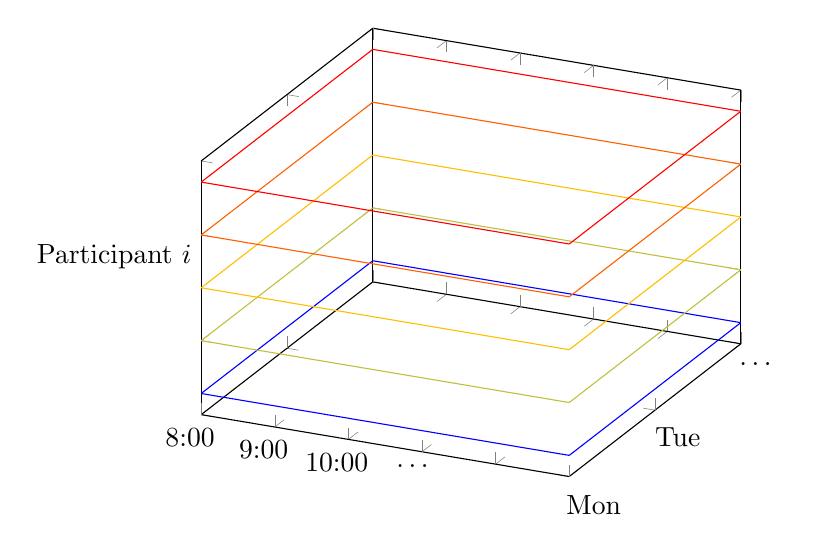
\begin{tikzpicture}

\begin{axis}[
  xlabel=, % Time,
  xticklabels={, 8:00, 9:00, 10:00, $\dots$},
  ylabel=, %Day,
  yticklabels={, Mon, Tue, $\dots$},
  zlabel=, %Participant,
  zticklabels = {, , ,Participant $i$}
  ]

  \foreach \i in {1,...,5}
     \addplot3[surf] coordinates { (0,0,\i) (1,0,\i) (1,1,\i) (0,1,\i) (0,0,\i)  };

  % \addplot3[surf] coordinates { (0,0,0) (1,0,0) (1,1,0) (0,1,0) (0,0,0)  };
  % \addplot3[surf] coordinates { (0,0,1) (1,0,1) (1,1,1) (0,1,1) (0,0,1)  };

\end{axis}


\end{tikzpicture}

%   \caption{Distributed university schedule.}
%   \label{fig:ScheduleSpace}
% \end{figure}


\end{document}

\documentclass[ThesisDoc]{subfiles}
\begin{document}

\section{Agents}
\green{Explicar qué son los agentes}
\medskip


\green{Poner algunas definiciones}
\medskip

An \emph{agent} has no generally accepted definition, but the idea is traced back
to the antique times. The survey of \cite[sec.~2.2]{PNoriega} gives several
definitions, proposed by different authors, ranging from philosophy to AI.

The notion of agent appears in Aristotle's works:
 ``entity that acts with a purpose, within a social context''.
The prætorian roman law defined an agent as
``a person who acts on behalf of a principal for
a specific purpose and under limited delegation of authority and responsibility''.

The earliest use of the term agent in AI was
``a program that is capable of executing an action vicariously''.
Later it was formulated as \emph{a computer system, which}
\begin{enumerate}
  \item has a degree of autonomy in determining its behavior,
  \item interacts with humans and or other agents,
  \item perceives the environment and reacts to it, and
  \item exhibits a goal directed behavior.
\end{enumerate}

\bigskip

There are three general approaches to defining/describing agents:
\begin{enumerate}
  \item \emph{Agent Theories} discuss what an agent \emph{is} and formalize
    it in mathematical form.
  \item \emph{Agent architectures} deal with the \emph{implementations}
    of the Agent Theories, physical (hardware) and/or logical (software).
  \item \emph{Agent languages} are software systems, that allow communication
    between the agents (including human/living ones).
\end{enumerate}


Many authors have thought of agents as \emph{logical theories}, that perceive
the environment as formulas, that are processed within or against those theories.
An agent is usually required to be capable of proactive behavior, not
just responses to environment changes. Some authors impose stronger demands upon
the agents, such as mobility, truthfulness, benevolence, rationality.

The most notable agent theory is the \emph{Beliefs-Desires-Intentions} (BDI) one,
that deduces agent's intentions (and the following sequence of actions)
from its desires (goals) and an uncertain image of the environment (beliefs).

\red{All this is taken from \cite[sec.~2.2]{PNoriega}, as mentioned before.
    In the original ,the information is taken from many different references,
    ¿should I put these specific references, or can I just leave the reference to
    the survey? }

The \cite{UAB-Thesis} and \cite{PNoriega} propose layered architecture,
capable of hosting different \emph{context logics}.
The logics are connected using \emph{bridge rules} and act as one.
The BDI theory can be implemented by creating the three contexts
(beliefs, intentions and desires) and the bridge rules.

\todo\red{: add another source.}


\bigskip
%%%%%%%%%%%%%%%%%%%%%%%%%%%%%%%%%%%%%%%%%%%%%%%%%%%%%%%%%%%%%%%%%%%%%%%%%%%%%%%%
\green{ Explicar qué es lo que tú entiendes por agente.}
\medskip

\noindent
One could summarize that an agent is primarily a computational entity (software),
where the hardware restriction is only be adequate for hosting the software
``consciousness''. In the rest, there is not much difference if an agent has
an actual physical body (\emph{mobile}), if it is emulated or was never intended.
The BDI theory, for example, allows to abstract existence of a body,
by seeing it as an actuator withing the environment, that \emph{tries} to
implement agent's current \emph{intention}.
The actual results of an interaction should not be taken as predefined, but rather
as probabilistic, observable through the \emph{beliefs}. As an example, one can
see a human being as an agent of its \emph{ego}, that determines the \emph{desires}.
As we all well know, not all the \emph{intention} always come out as expected.
It depends, of course, on how general one understands intention, but whether
it's an intention to go to Mars or to lift a pen, there is always a degree of
uncertainty. Our brain, as an actuator, transforms motion intentions into
neuronal signals, even if there destination was severed or the neural connections
were damaged; there is no way of knowing the results of intention implementation
except from new information.

\bigskip

\noindent
An agent should be capable of:
\begin{enumerate}
  \item \emph{autonomous} and \emph{goal directed} behavior,
  \item perception of and interaction with the environment,
  \item communication with other agents (including humans).
\end{enumerate}

\todo\red{: this is basically a repetition}

\subsection{Solving CSPs with Multiagent Systems}
%%%%%%%%%%%%%%%%%%%%%%%%%%%%%%%%%%%%%%%%%%%%%%%%%%%%%%%%%%%%%%%%%%%%%%%%%%%%%%%%
\green{Explicar cómo se pueden resolver los CSP con agentes}
\medskip

Multiagent Systems (MAS) have been successfully used to solve
different \emph{constraints satisfaction problems} \cite{MAS, MAS-Survey}.
Each problem variable is given to an agent, that would try to set its value,
avoiding contradictions with the values of its ``neighbouring'' agents.
There are different methods and techniques for implementing agents behavior.

One of the simplest methods consists in taking all possible variable domain values
and eliminating the values, that are in contradiction with the neighbors.
The process results in a solution if when all the agents have exactly one
possible value; or it fails if any of the agents runs out of the possible
values to propose. A natural question arises: in what order should the agents
prune their domains?
It can be resolved by assigning a distinct comparable priority value to each agents.
In such case a value should be excluded only if neighbor's priority exceeds own priority.
Combined with \emph{backtracking} technique, it guarantees finding a solution,
if it exists.

\noindent
An agent $a_i$
\begin{enumerate}
  \item controls variable $v_i$ with a finite $\domain~v_i =
        \{{\dot v}^i_j\}_{j=1}^{N_i}$, can set it's value ${\dot V}_i$,
  \item has sets of possible ${\tilde V}_i$ and excluded ${\tilde V}_i^-$ values,
  \item has priority $p$.
\end{enumerate}

\noindent
In the beginning each agent assigns
\begin{align*}
  &{\tilde V}_i   &&\leftarrow \domain~v_i       && \textit{(any domain value is possible)} & \\
  &{\tilde V}_i^- &&\leftarrow \{\}              && \textit{(no excluded values at start)}  &\\
  &{\dot V}_i     &&\leftarrow \pop~{\tilde V}_i && \textit{(pop first possible value and assign it to the variable)} &\\
\end{align*}

Every time current value ${\dot V}_i$ is assigned, an agent must notify its
neighbors about it with a \emph{proposal} message, containing the value.
The interactions between agents are heavily based on their priority and are
defined for pairs, where one of the agents always has a higher priority.

Agents communications can be divided in two groups, each depending on the relative
priorities.
\begin{enumerate}
  \item Testing constraints of the \textbf{lower priority} agents by the
    \textbf{higher priority} ones.
    Each agent must notify its neighbors on every value assignment and wait
    for a confirmation from the higher priority ones. If any of them responds
    negatively, the agent must try next \emph{possible} value from ${\tilde V}_i$.
    In case that possible values have ended (${\tilde V}_i = \emptyset$), the agent
    must notify its direct superior (the neighbor with the next highest priority)
    about it, starting the \emph{backtracking}.
  \item Backtracking permits to exit dead-end solution branches, thus allowing
    to check \emph{every possible values combination} with limited resources.

    As written in previous item, the backtracking process starts when an agent
    finds itself without possible values to assign. It has searched all of its
    domain, but no solution to its part of a problem exists. Therefore it is
    necessary that a higher priority agent changes its value. It is better to
    keep the process ordered and the next priority agent is a rational choice
    for a supervisor.

    Upon a notification about solution incoherence, the supervisor
    must try to change its value ${\tilde V}_s$ and add the old one to the
    excluded set ${\tilde V}_i^-$.
    If neither this agent has more possible values to assign, it should propagate
    backtracking request to its own supervisor, and so on. Otherwise, it should
    demand its subordinates to reset their ${\tilde V}_*$ and ${\dot V}_*$ states
    before changing its value. New \emph{possible values} sets are formed, considering
    the excluded values: ${\tilde V}_* = \domain~v_* \setminus {\tilde V}_*^-$.
    Backtracking request by the \emph{top priority} agent means that no solution
    could be found.
\end{enumerate}

The \textbf{stop criteria} is the lack of negotiation activity, that signalizes
that all the values assignations have been confirmed, thus a solution, satisfying
the constraints, was found.

\bigskip
%%%%%%%%%%%%%%%%%%%%%%%%%%%%%%%%%%%%%%%%%%%%%%%%%%%%%%%%%%%%%%%%%%%%%%%%%%%%%%%%

\noindent
There are various extensions of the method that improve its speed.

One of such techniques is \red{don't remember [I've lost the reference]}.
It can be used when the agents control several variables. It consists in
aggregating variables into negotiation one-by-one, finding \emph{partial solutions}
at each step, until all the variables are aggregated and the final solution
is found. When a (partial) solution cannot be found for a newly aggregated
variable, a process, similar to backtracking, is used to change previous
partial solutions.

A good example of a problem, that is solved much faster this way, is
\emph{n-queen} problem. If one considers the position variable
$\left< x,y \right>$ as two variables, owned by the same agent, the queens
can be positioned first by rows and then by columns, or vice versa. Anyway,
the number of combinations to consider is reduced greatly, thus accelerating
solution search.

There is, for example, a technique, that manipulates agents priorities,
decreasing the priorities of the agents that have fallen back in the backtracking
procedure and rising the priorities of their subordinates. It reduces the
the negotiation time, by shortening the subordinates chains, that are
revised on every backtrack event, of frequently changing agents.

\bigskip

\noindent
In \cite{MAS-Survey} the MAS are classified by two properties of the agents,
that form the system: heterogeneity and communications.
The classification is presented in figure \ref{table:MAS-Table}. It denotes
that CSPs are usually solved by \emph{heterogeneous communicating} agents.
problems is

\begin{table}
  \label{table:MAS-Table}
  \centering
  \begin{tabular}{P{0.1\textwidth} P{0.3\textwidth}|P{0.4\textwidth}}
    & \centering Homogeneous & Heterogeneous \\
    \begin{minipage}{0.1\textwidth}
      \rotatebox[origin=tr]{90}{Non-Communicating}
    \end{minipage}
                      & \begin{minipage}{0.3\textwidth}
                        \footnotesize \begin{itemize}[leftmargin=5px, rightmargin=0px]
                          \item Reactive vs. deliberative agents
                          \item Local or global perspective
                          \item Modeling of other agents' states
                          \item How to affect others
                        \end{itemize}\end{minipage}
                      & \begin{minipage}{0.4\textwidth}
                        \footnotesize\begin{itemize}[leftmargin=10px, rightmargin=0px]
                          \item[]
                          \item Benevolence vs. competitiveness
                          \item Fixed vs. learning agents (arms race, credit assignment)
                          \item Modeling of others’ goals, actions, and knowledge
                          \item Resource management (interdependent actions)
                          \item Social conventions
                          \item Roles
                          \item[]
                        \end{itemize}\end{minipage}
                      \\\hline
                      % \\ \rule{0pt}{4ex}\\\hline\\\rule{0pt}{4ex}
    \begin{minipage}{0.1\textwidth}
      \rotatebox[origin=tr]{90}{Communicating}
    \end{minipage}
                      & \begin{minipage}{0.3\textwidth}
                        \footnotesize\begin{itemize}[leftmargin=5px, rightmargin=0px]
                          \item Distributed sensing
                          \item Communication content
                        \end{itemize}\end{minipage}
                      & \begin{minipage}{0.4\textwidth}
                        \footnotesize\begin{itemize}[leftmargin=10px, rightmargin=0px]
                          \item[]
                          \item Understanding each other
                          \item Planning communicative acts
                          \item Benevolence vs. competitiveness
                          \item Negotiation
                          \item Resource management (schedule coordination)
                          \item Commitment/decommitment
                          \item Collaborative localization
                          \item Changing shape and size
                        \end{itemize}\end{minipage}
  \end{tabular}
  \caption{Issues arising in the various scenarios as reflected in the literature
          \cite[Table~2]{MAS-Survey}.}
\end{table}


\subsection{Negotiating Agents}
%%%%%%%%%%%%%%%%%%%%%%%%%%%%%%%%%%%%%%%%%%%%%%%%%%%%%%%%%%%%%%%%%%%%%%%%%%%%%%%%
\label{sec:NegotiatingAgents}
\green{ Explicar qué es lo que tú entiendes por agente.}
\medskip

A \emph{negotiation} is a process of communication between heterogeneous agents with a
goal of finding such a configuration of variables assignations, that all the
agents involved agree upon it. The results and the time of a negotiation depend
on agents \emph{cooperation}. The latter implies that agents must pursue a
\emph{common goal}, rather than be selfish; it can be formulated as
``the good of many outweigh the good of the one''.


\bigskip

\noindent
In this thesis the following definition of a class of agents is used:
a \textbf{negotiating agent} is an isolated proactive computational entity,
capable of sending and receiving messages.
The \emph{isolation} denotes that agents' variables are protected
from outside access; messaging is the only way an agent can be interacted with.
The \emph{pro-activity} implies a capacity of acting asynchronously,
with no ``external'' cause.


\medskip

An agent is defined by it's behaviour --- the combination of its
\emph{proactive} and \emph{reactive} (message handling) functions.

\begin{flalign*}
  &\behaviour = \left< \behaviour_\act, \behaviour_\react \right>\\
  &\behaviour_\act   : \state \mapsto \action \\
  &\behaviour_\react : \state \times \msg \mapsto \action
\end{flalign*}

Therefore two agents with same behaviour functions should be considered two instances
of the same agent. In must be noted, that all the diference in the behaviour of
two instances is produced by the differences in the states
(both agent's internal state and the environment's one).

\medskip

The agents, participating in a negotiation, are considered \emph{heterogeneous}
(to any degree: from complete heterogeneity to homogeneity).
In order to generalize some agents behaviour, \textbf{negotiation roles} are introduced.
A role describes whom or what an agents represents in the negotiation and
defines \emph{behaviour archetype} --- the rules to build
agent's \emph{behaviour functions}, given some \emph{role-specific} knowledge.

The agents must use a common \emph{communication protocol}, to ensure
understanding between agents of the same or different roles.


%%%%%%%%%%%%%%%%%%%%%%%%%%%%%%%%%%%%%%%%%%%%%%%%%%%%%%%%%%%%%%%%%%%%%%%%%%%%%%%%
% \subsection{Agents Implementation}

Agents are implemented using \emph{Software Transactional Memory} (STM)
\cite{STMCode07} --- a promising concurrency paradigm.
They are executed in two computational threads:
one for message handling and another for proactive action.

\medskip

\noindent
Agent's behavior is flexible and may be changed during agent's lifetime.
As it was mentioned before, it is determined by \emph{message handling} and
\emph{action} functions.
Any complex behaviour would require the agent to have some \emph{mutable}
internal \emph{states}, where it could store some information,
thus remembering it throughout behaviour executions.
The only restriction is that states interface must be fixed for type safety
(only the interface, not the underlying data).


Each agent also has two system states: the \emph{run state} and special \emph{shared
  state}, called \emph{status}. The run state controls agent's execution
(and termination), while the status is monitored by the respective controller.
Agents have three \emph{run states}: ``Paused'', ``Running'' and ``Terminate''.
The first two states should control pro-action;
setting the last one should cause all agent's processes to stop.
The \emph{status}es are further described in section \ref{agentControllers}.

\medskip

To ensure agents isolation, the direct interactions are restricted;
an agent only exposes its communication interface through \emph{agent reference}.

Using this interface, one can simply \emph{send} a message to an agent,
or one can \emph{ask} for some \emph{expected response}, corresponding to the message sent.
Agents have separate handler functions for theese two cases.

% \medskip

% All behavior functions
% accept two arguments:
% \begin{enumerate}
% \item the agent's \emph{inner interface}, that provides
%   control over agent's own behavior and lifetime;
% \item agent's \emph{internal state}.
% \end{enumerate}

% \subsubsection{Negotiation}
%
%
% A negotiation has a \emph{classes pool}, distributed between the agents.
% A class $\left< d, g, p, r, \bar d, t, t \right>$ is known to agents,
% representing $g$, $p$ and $r$.
%
% Negotiations are organized by special kind of agents --- \emph{controllers}.
%
% \red{TODO}






\subsection{Controllers}
\red{rename: ``Controller'' => ``Observer''}

The controllers create new negotiating agents, and monitor their \emph{status}es
over their lifetimes. Controllers also provide communication references for the
agents they control. In order to facilitate references sharing, the controllers
are restricted to a single \emph{role} for it's agents.

Controllers have hierarchical structure, starting with the \emph{root
  controller}. The orders received by \emph{root} are propagated to
the underlying controllers.

\medskip

As mentioned before, negotiating agents have a special state,
called \emph{status}, that is monitored by the controllers. Apart
from receiving agents' errors, the \emph{status}es are used to
extract the \emph{distributed solution} from the agents.
This is done using ``Waiting'' and ``Locked'' statuses.

The agents set ``Waiting'' status when a suitable solution is found,
and the corresponding controller waits for all of its subjugated
agents to set it. When it is done, the controller sends ``Lock''
command to the agents and notifies the \emph{parent controller}.
When the \emph{root controller} receives ``Lock'' notifications from
all the controllers, it sends ``Collect'' order. On that order, the controllers
extract the solution parts (guarded in the statuses) and propagate them up to
the root.


\end{document}

%\documentclass{article}


%\usepackage{hyperref, float, amsmath}
%\usepackage{tikz, ifthen, xcolor}
%\usepackage[english]{babel}

%\usetikzlibrary{fit, calc, arrows, shapes}

%\newcommand{\red}[1]{{\color{red} #1}}


%\begin{document}

\def\coh{\mathrm{coh}}
\def\cohi{\mathrm{\widetilde{coh}}}


\section{Coherence and Contexts}
\label{section:coherence}


Within an agent, the coherence is established over \emph{information graphs},
containing the assessed candidate's classes and \emph{context-specific
  knowledge} --- an \emph{information graph}, that holds the information,
already known/accepted by the agent.

The coherence concept and the idea of coherence-based agents
where taken from \cite{UAB-Thesis}, but the contexts and
coherence assessment were modified.

In \cite{UAB-Thesis} the best partition $\mathcal{A}$ \red{(called \emph{candidate} in this thesis)}
is obtained by an information graph $\mathcal{V}$, considering both
$\mathcal{A}$ and $\mathcal{V} \backslash \mathcal{A}$, as shown in figure
\ref{fig:UAB-partition}. The graph $\mathcal{V}$ is obtained by joining
contexts' graphs \cite[62]{UAB-Thesis}.

\begin{figure}[h]
  \label{fig:UAB-partition}
  \centering
  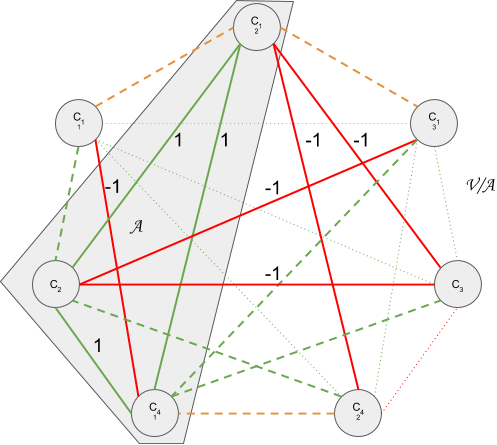
\includegraphics[width=0.5\textwidth]{img/UAB-splitting.png} % scale=0.5
  \captionsetup{singlelinecheck=off}
  \caption[caption]{ The coherence of partition $\mathcal{A},\mathcal{V}\backslash\mathcal{A}$
            is calculated in \cite{UAB-Thesis} as $
            \dfrac{ \text{\green{\emph{consistent}} relations in } \mathcal{A}
                  + \text{\red{\emph{inconsistent}} relations between }
                          \mathcal{A} \text{ and } \mathcal{V}\backslash\mathcal{A}}
                  {\text{total relations in } \mathcal{V}}$.
            \medskip\\ %\hspace{\textwidth}
            On the image above, the information graph $\mathcal{V}$ consists of
            classes $C_1,\dots,C_4$, also there are three possibilities for
            class $C_1$ placement and two for class $C_4$.

            A relation is
            \begin{itemize}[leftmargin=3cm]
              \item[\red{\emph{inconsistent}}], if two classes intersect in time;
              \item[\yellow{\emph{same class}}], if two classes differ only by time;
              \item[\green{\emph{consistent}}], otherwise.
            \end{itemize}

            Coherence of the partition is $\frac{|1| \cdot 3 + |-1| \cdot 5}
                                                {17} \approx 0.47$.
          }
\end{figure}


In this thesis, a different aproach is taken. The initial information graph,
composed of \emph{classes propositions}, is passed to a \emph{splitting} context,
that generates all posiible \emph{acceptable} (by the splitting context) sub-graphs,
called \emph{candidates} (as it will be shown in \emph{Beliefs} context).

Each candidate is propagated through the contexts in the established
order. At each context it gets assessed and the result is compared
against \emph{context-specific threshold}. If passing threshold test,
the candidate is sent to the next context, otherwise it is marked as failed
(providing a reason) and is propagated no further. In both cases the coherence
value is guarded alongside the candidate.

Thus a context in this thsis serves as \emph{candidates} filter.
\medskip

\noindent
A \emph{context} represents an aspect for optimization/restriction, considered
by an agent. It defines context-specific information and relations over the
information graph, with the corresponding combination functions. There are
two types of relations: \emph{binary} and over the \emph{whole graph}. The former ones
are applied to every pair of nodes and the results are combined by
\emph{binary fold functions} (one combines the results of the same relation
and the other combines the latter results). The whole-graph relations' values are
combined by the corresponding \emph{whole-graph fold function}. In the end the
combined values of both relations types are merged into the result by
\emph{combined merge function}. All the combination functions are defined at
contexts.

\begin{figure}[h]
  \centering
  \fbox{ 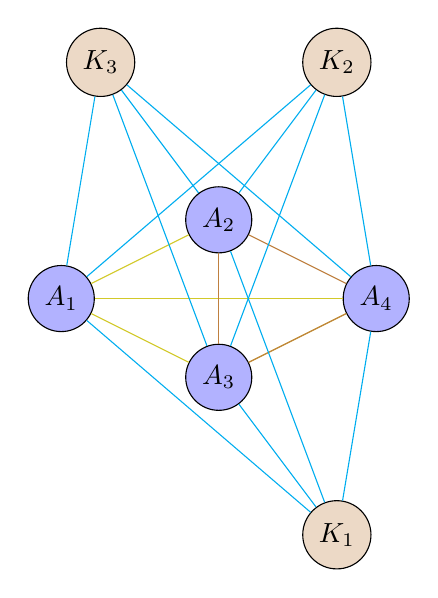
\begin{tikzpicture}

\tikzstyle{assessed}=[draw, circle, fill=blue!30];
\tikzstyle{innerKn}=[draw, circle, fill=brown!30];

\node[assessed] (a1) at (-2,0) {$A_1$};
\node[assessed] (a2) at (0, 1) {$A_2$};
\node[assessed] (a3) at (0,-1) {$A_3$};
\node[assessed] (a4) at (2, 0) {$A_4$};

\node[innerKn] (k1) at (1.5,-3) {$K_1$};
\node[innerKn] (k2) at (1.5, 3) {$K_2$};
\node[innerKn] (k3) at (-1.5,3) {$K_3$};

\begin{scope}[color=yellow!80!black]
 \foreach \i in {1,...,4}
  \foreach \j in {\i,...,4}{
   \ifthenelse{\NOT \(2 = \i \AND \(4 = \j \OR 3 = \j\)\) }
              { \draw (a\i) -- (a\j); }
              {}}
\end{scope}

\begin{scope}[color=brown]
 \foreach \i in {2,3,4}
  \foreach \j in {\i,...,4}
   \draw (a\i) -- (a\j);
\end{scope}

\begin{scope}[color=cyan]
 \foreach \i in {1,...,3}
  \foreach \j in {1,...,4}
   \draw (k\i) -- (a\j);
\end{scope}

\end{tikzpicture}

 }
  \caption{Binary relations within an information graph. One can
           distinguish the relations between the assessed information pieces
           and the relations between assessed and the known ones.
          }
\end{figure}


\subsection{Internal Contexts}

An internal context requires no knowledge from other agents.
The combined coherence of all the internal contexts is called
\emph{inner coherence} and is denoted as $\cohi$.

% % % % % % % % % % % % % % % % % % % % % % % % % % % % % % % % % % % % % % % %
\subsubsection{Capabilities}

Represent \emph{strong} restrictions, imposed by the institution.
All the relations should yield
\begin{itemize}
  \item [1], if the restriction is satistied;
  \item [0], otherwise.
\end{itemize}

Institution restrictions:
\begin{itemize}
\item \textbf{Group:} the candidate has the correct amount of classes for each
  discipline inscribed.
\item \textbf{Professor:} can teach every discipline assigned.
\item \textbf{Classroom:} has enough capacity and meets all special requirements.
\end{itemize}

An agent should be keeping the capabilities of known agents, to avoid creation
of unacceptable classes.

\begin{figure}[h]
  \centering
  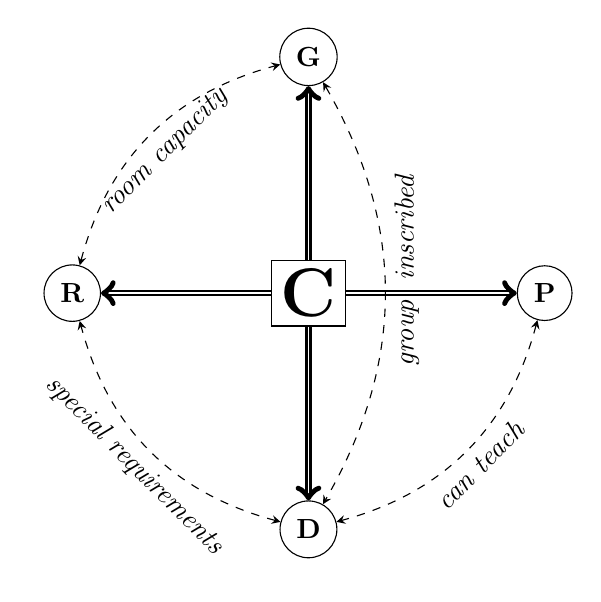
\begin{tikzpicture}
 
\edef\r{3cm}

\node[draw]         (C) at (0,  0) {\textbf{\Huge C}};
\node[draw, circle] (G) at (0, \r) {\textbf{G}};
\node[draw, circle] (P) at (\r, 0) {\textbf{P}};
\node[draw, circle] (D) at (0,-\r) {\textbf{D}};
\node[draw, circle] (R) at (-\r,0) {\textbf{R}};

\foreach \i in {(G),(P),(D),(R)}
 \draw[->, thick, double] (C) -- \i;

\def\data{ P/D/can teach
         , D/R/special requirements
         , R/G/room capacity
         , G/D/\quad~ group~~inscribed
         }

\foreach \i/\j/\k in \data
 \draw[<->, >=stealth, dashed] (\i) to[bend left
                                      ,edge node={node [sloped, below] {\emph{\k}}}]
                               (\j);


\end{tikzpicture}
  \caption{Capabilities required to form a \emph{class}.}
  \label{fig:capabilities}
\end{figure}


% % % % % % % % % % % % % % % % % % % % % % % % % % % % % % % % % % % % % % % %
\subsubsection{Beliefs (Time Consistency)}

Asserts that all the classes (concerning the assessing agent), are consistent in
time (do not intersect). This context is a splitting one, it uses the time
consistence relation to generate all possible time-consistent candidates from
given classes. It's internal knowledge should hold \emph{classes pool}, that
would be used for candidates generation via \emph{graph splitting}.
\\

The \emph{time consistence} relation yields following values:
\begin{itemize}[leftmargin=2cm]
  \item[-1], if two classes intersect in time (are inconsistent);
  \item[0], if two classes differ only by time
            (while have same discipline, group, professor and classroom);
  \item[1], otherwise (are consistent).
\end{itemize}


The splitting process uses context's relation \emph{aggregation} strategy.

\begin{align*}
  \mbox{Let } & C=\lbrace c \rbrace \text{ be the \emph{classes pool}}.\\
            ~ & A_i=\lbrace a_i \rbrace \text{ be a set of \emph{acceptable candidates},
                                         composed of } i \text{ classes.}\\
            ~ & A=\bigcup\limits_{i} A_i \text{ be a set of \emph{acceptable candidates}}.
\end{align*}

\begin{enumerate}
  \item Each single-class candidate is acceptable:
    $A_1 = \lbrace [ c ] ~||~ \forall ~ c \in C \rbrace$.
  \item Form $A_2$ by extending each candidate $[c'] = a_1 \in A_1$ with $c \in C$,
    if and only if $c'$ and $c$ are \emph{consistent in time}.
    If $A_1 \not= \emptyset$, then try to form $A_2$.
  \item[\vdots]
  \item[i.] Form $A_i$ by extending each candidate $[c'_1, \dots, c'_{i-1}] = a_{i-1}
    \in A_{i-1}$ with $c \in C$, if and only if $\forall c' \in a_{i-1}, ~c'$
    and $c$ are \emph{consistent in time}.
    If $A_i \not= \emptyset$, then try to form $A_{i+1}$.
   \item[\vdots]
   \item[n.] $A_n = \emptyset \implies$ all the \emph{acceptable candidates}
     were generated. Done.
\end{enumerate}


\begin{figure}[h]
  \label{fig:splittingCtx}
  \def\sfwidth{0.24\textwidth}
  \begin{subfigure}[b]{\sfwidth}
    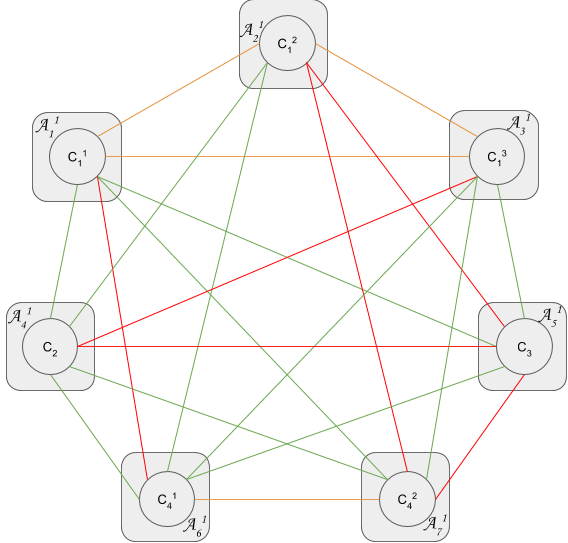
\includegraphics[width=\textwidth]{img/split-1-class.png}
    \caption{All single-class candidates are acceptable.}
  \end{subfigure}
  \begin{subfigure}[b]{\sfwidth}
    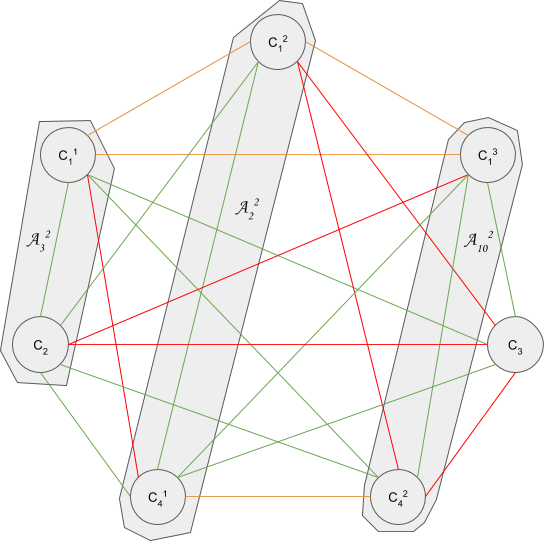
\includegraphics[width=\textwidth]{img/split-2-class_1.png}
    \caption[caption]{$\begin{aligned}
              A_3^2    &= A_1^1 + A_4^1\\
              A_2^2    &= A_2^1 + A_6^1\\
              A_{10}^2 &= A_3^1 + A_7^1
            \end{aligned}$}
  \end{subfigure}
  \begin{subfigure}[b]{\sfwidth}
    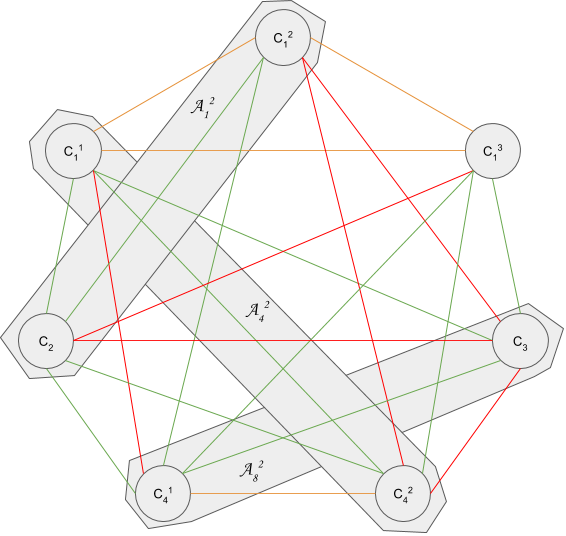
\includegraphics[width=\textwidth]{img/split-2-class_2.png}
    \caption[caption]{$\begin{aligned}
              A_1^2 &= A_2^1 + A_4^1\\
              A_4^2 &= A_1^1 + A_7^1\\
              A_8^2 &= A_5^1 + A_6^1
             \end{aligned}$}
  \end{subfigure}
  \begin{subfigure}[b]{\sfwidth}
    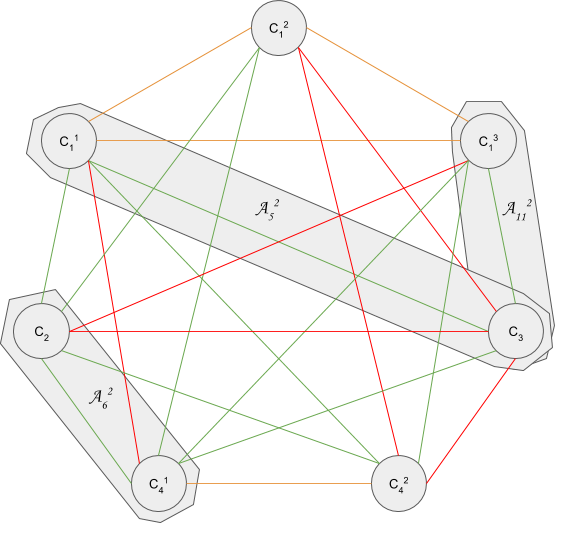
\includegraphics[width=\textwidth]{img/split-2-class_3.png}
    \caption[caption]{$\begin{aligned}
              A_5^2    &= A_1^1 + A_5^1\\
              A_{11}^2 &= A_3^1 + A_5^1\\
              A_6^2    &= A_4^1 + A_6^1
             \end{aligned}$}
  \end{subfigure}
\\
  \begin{subfigure}[b]{\sfwidth}
    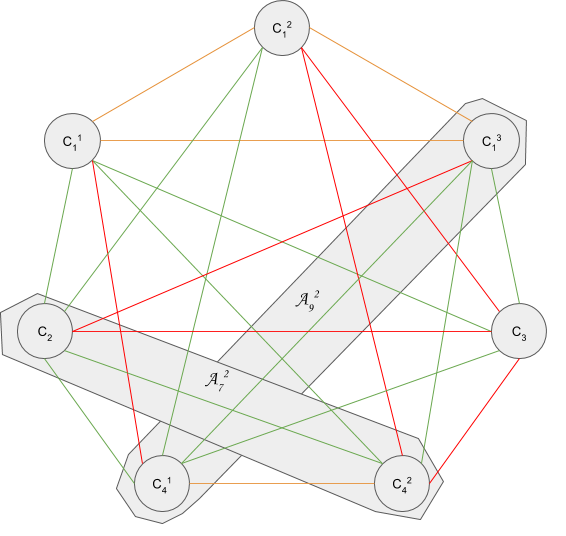
\includegraphics[width=\textwidth]{img/split-2-class_4.png}
    \caption[caption]{$\begin{aligned}
              A_7^2 &= A_4^1 + A_7^1\\
              A_9^2 &= A_3^1 + A_6^1
             \end{aligned}$}
  \end{subfigure}
  \begin{subfigure}[b]{\sfwidth}
    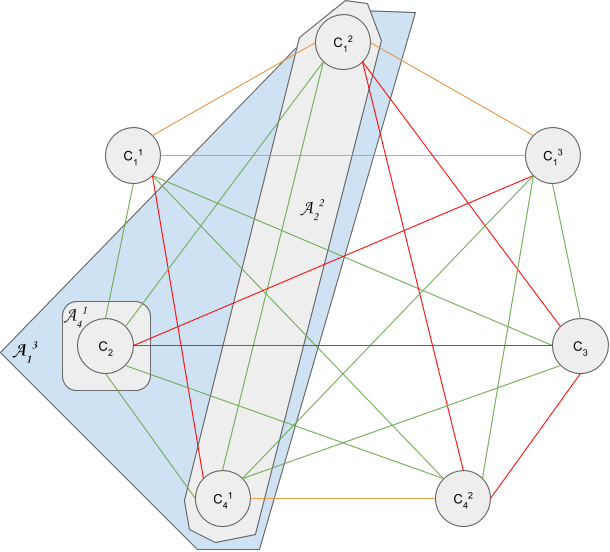
\includegraphics[width=\textwidth]{img/split-3-class_1.png}
    \caption[caption]{$\begin{aligned}
              A_1^3 &= A_2^2 + A_4^1\\
                    &= A_1^2 + A_6^1\\
                    &= A_6^2 + A_2^1
              \end{aligned}$}
  \end{subfigure}
  \begin{subfigure}[b]{\sfwidth}
    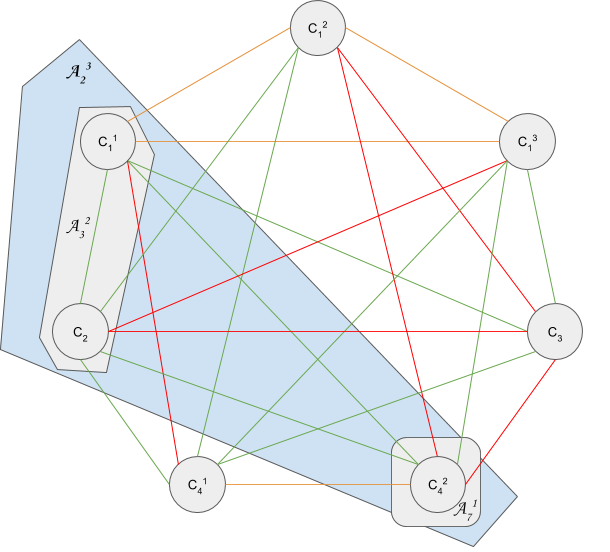
\includegraphics[width=\textwidth]{img/split-3-class_2.png}
    \caption[caption]{$\begin{aligned}
              A_2^3 &= A_3^2 + A_7^1\\
                    &= A_4^2 + A_4^1\\
                    &= A_7^2 + A_1^1
              \end{aligned}$}
  \end{subfigure}
  \begin{subfigure}[b]{\sfwidth}
    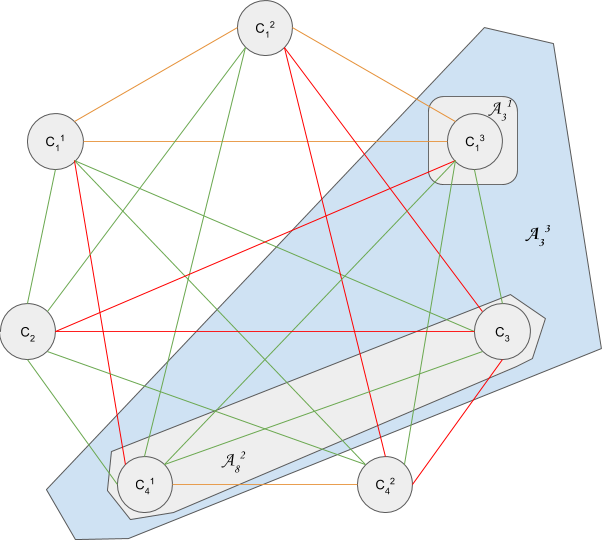
\includegraphics[width=\textwidth]{img/split-3-class_3.png}
    \caption[caption]{$\begin{aligned}
              A_3^3 &= A_8^2    + A_3^1\\
                    &= A_{11}^2 + A_6^1\\
                    &= A_9^2    + A_5^1
              \end{aligned}$}
  \end{subfigure}

  \caption{Information graph \emph{splitting} example. The graph is the same
           as in figure \ref{fig:UAB-partition}.
           There are in total \textbf{7}  1-class candidates,
                                    \textbf{11} 2-class candidates and
                                    \textbf{3}  3-class candidates.}
\end{figure}



% % % % % % % % % % % % % % % % % % % % % % % % % % % % % % % % % % % % % % % %
\subsubsection{Obligations}

The obligations determine custom \emph{strong restrictions} over the classes.
As in the case of \emph{capabilities}, the obligation relations must yield a
boolean result.

Possible \emph{obligation relations} examples: maximum classes per day,
lunch recess time, lower/upper class time limit, two classes must/cannot follow etc.

\red{At the moment there are no obligations used (but they are supported).}

% % % % % % % % % % % % % % % % % % % % % % % % % % % % % % % % % % % % % % % %
\subsubsection{Preference}

The preferences define \emph{weak restrictions}. The relations values might be any
value within $[0,1]$ interval. To avoid overrestrictions, this context's \emph{threshold}
should decrease with time.

\red{Possible preferences}

% % % % % % % % % % % % % % % % % % % % % % % % % % % % % % % % % % % % % % % %
\subsection{External}

The external context asks counterparts an \emph{opinion} about a candidate.
An opinion is the \emph{inner coherence} of the agent being asked.

\red{todo: images from g-drive ``ThesisCandidatesCommonGoal''}

%\end{document}

\documentclass[ThesisDoc]{subfiles}
\begin{document}

\providecommand{\rootdir}{.}


\def\domain{\mathrm{domain}}

\def\domain{\mathrm{domain}}
\def\pop{\mathrm{pop}}

\def\behaviour{\mathrm{behaviour}}
\def\act{\mathrm{act}}
\def\react{\mathrm{react}}
\def\state{\mathrm{state}}
\def\action{\mathrm{action}}
\def\msg{\mathrm{message}}

\def\coh{\mathrm{coh}}
\def\cohi{\mathrm{\widetilde{coh}}}
\def\rel{\mathrm{rel}}
\def\fold{\mathit{fold}\,}

\def\restrC{\accentset{C}{\xi}}
\def\restrT{\accentset{T}{\xi}}
\def\restrS{\accentset{S}{\xi}^p_i}
\def\restrW{\accentset{W}{\xi}^p_i}

\def\ctx{\mathit{ctx}}
\def\codom{\mathrm{codomain}}
\def\maybe{\mathrm{Maybe\,}}


\section{Problem Formalization}
\label{sec:ProblemFormal}


Let \begin{itemize}
\item $D=\{d_i\}$ be set of \emph{disciplines}.
  A discipline may be seen as class descriptor, it contains
  academic program name and information about special requirements,
  such as laboratory equipment.
\item $G=\{g_i\}$ be set of \emph{groups}.
  A group unites some students. In this thesis it is assumed that
  \textbf{each student belongs strictly to one group}.
  A group has a set of disciplines, that it is obliged to take by an
  academical program: $D^G_i$.
\item $P=\{p_i\}$ be set of \emph{professors}.
  Each professor can teach a set of disciplines, that is determined
  by the institution.
  % There are two kinds of professors:
  % \emph{full-time} and \emph{part-time}. The difference is that the
  % latter have more flexible obligations, while the former have preference
  % in classes assignment. All professors are treated in the same manner;
  % \emph{part-time} agents have stronger obligations ... \todo\red{: it should be
  % written elsewhere.}
\item $R=\{r_i\}$ be set of \emph{classrooms}.
  A classroom has two properties: capacity and special equipment installed.
\item $\bar D=\{\bar d_i\}$ be the set of working \emph{days}.
\item $\bar T=\{\bar t_i\}$ be \emph{discrete time} (limited by working hours).
\item $\mathrm{cc} \sim \left< d, g, p \right>$ be a \emph{class core}, that
      links group $g$ with professor $p$ through a \emph{possible class} for
      discipline $d$.
\item $ c \sim \left< \mathrm{cc}, r, \bar d, \bar t_b, \bar t_e \right> $
      be a \emph{class} --- an ``instance'' of some \emph{class core}, that has
      certain day, time (beginning \& end) and room assigned.
\item $\{\restrC\}$ be the restrictions over the classes.
      $\restrC : c \mapsto \mathrm{Bool}$
\item $\restrT$ be the \emph{time-consistency} restriction, that ensures
  classes non-intersection for each participant.
      $\restrT : c \mapsto c \mapsto \mathrm{Bool}$
\item $\{\restrS\}$ be the rest of strong restrictions, or \emph{obligations},
      of participant $p$.
      $\restrS : \{c\} \mapsto \mathrm{Bool}$
\item $\{\restrW\}$ be the weak restrictions, or \emph{preferences}, of participant $p$.
      In order to avoid overrestrictions, the preferences should weaken with time.
      $\restrW : \tau \mapsto \{c\} \mapsto (0,1]$
\item $\tau$ be \emph{negotiation time}. $\tau \in \mathbb{N}$
\end{itemize}
\medskip

\noindent
A \emph{candidate to partial solution} $\tilde{c}_a^k$ (just \emph{candidate} further)
is a set of classes $\{c_a^*\}$, that:
\begin{enumerate}
  \item Complies with \emph{class restrictions}: \\
    $$\forall c_a^* \in \tilde{c}_a^k \implies \restrC(c_a^*) = \true$$
  \item Complies with \emph{time-consistency} restriction: \\
    $$\forall c_a^*, c_a^\circ \in \tilde{c}_a^k ~|~ c_a^* \not= c_a^\circ \implies
      \restrT(c_a^*, c_a^\circ) = \true$$
  \item Is \textbf{proposed by a group}: $a = g_i$.
  \item Has enough classes for each discipline, that group $g_i$ is enrolled.
        Doesn't have excess classes or classes for other groups:
        $$\tilde{c}_i^k = \bigcup\limits_{d \in D^G_i}
                            \lbrace c_i^n \rbrace_d ~|~ \mathsmaller{
                                \mathrm{discipline}(c_i^n) = d;~
                                \sum\limits_n \mathrm{time}(c_i^n) =
                                              \mathrm{time}(d)   }$$

\end{enumerate}
\bigskip

\noindent
A solution to the scheduling problem is a valid union of \emph{all} partial solutions.



\begin{figure}[h]
  \centering
  \resizebox{\textwidth}{!}{
    \subfile{\rootdir/img/ScheduleHypercube/GRPT.tikz}
  }
  \caption{Schedule 4-dimensions space. Each \emph{group} $G_i$,
          \emph{professor} $P_k$ and \emph{classroom} $R_j$ has a
          \underline{timetable} (Day $\times$ Time) of its own.}
  \label{fig:ScheduleHypercube}
\end{figure}

\end{document}

\section{Proposed Solution}
\green{Explicar la solución de manera informal, y después ...}
\medskip


\def\ctx{\mathit{ctx}}
\def\codom{\mathrm{codomain}}
\def\maybe{\mathrm{Maybe~}}


\noindent
The solution to \emph{university classes scheduling problem} (UCSP), proposed
in this thesis, is based on a \emph{negotiation} within a \emph{Multiagent System},
properly discussed in section \ref{sec:NegotiatingAgents}.
Decision processes of the negotiating agents are \emph{coherence-based}
that are discussed in section \ref{sec:coherence}.
Here follows a short summary:
\begin{itemize}
  \item Each agent represents a \emph{professor}, a \emph{group} or a \emph{classroom},
    that are to be put schedule together.
  \item Each agent has internal states, accessible only to it, that hold
    agent's contexts. The contexts contain agent-specific information and constraints.
    Some context variables may/must change during a negotiation.
  \item Agents can interact only using communication: by sending and receiving messages.
  \item Agents can process messages and execute another action at the same time.
  \item Agent's goal is to find a configuration of classes, that complies with
    all the restrictions, contained in the contexts.
  \item Agent's decision process is based on the coherence between the existing
      \emph{classes proposals}, called \emph{classes pool}, and its contexts.
      The classes proposals and one of the contexts, specifically its constraints,
      are used to form valid configurations of classes, called \emph{solution candidates}.
      The candidates are then propagated through the rest of the contexts in the
      defined order. At each context the candidate's coherence is assessed using
      context-specific constraints and the established value is compared against
      a context-specific threshold in order to be propagated further.

      The final decision is based on a set of \emph{acceptable candidates}, that
      have complied successfully with all the contexts' restrictions. It should
      choose whether to:
      \begin{itemize}
        \item add new classes proposals (and remove some old), in case no
          acceptable candidate was found;
        \item select the candidate with maximum coherence as the solution and
          request acceptance confirmation from the ``neighboring'' agents.
      \end{itemize}

  \item The contexts are divided into
    \begin{itemize}[leftmargin=2cm]
      \item[Internal:] define different aspects of agent-specific \emph{internal coherence}
      with solution candidates:
        \begin{enumerate*}[1)]
          \item capabilities,
          \item time consistency,
          \item obligations,
          \item preferences.
        \end{enumerate*}
      \item[External:] communicates with the ``neighboring'' agents and fetches
        their opinions about the candidates, thus cooperating towards the
        \emph{common goal}.
    \end{itemize}
 \end{itemize}

External context combines the \emph{internal coherences} of a candidate,
assessed by the agents, involved in the candidate's underlying classes.
The combination is done, giving no priority to any of the agents,
thus creating an important property:
\begin{displayquote}
  Given a candidate $\tilde{c}$, each agent $g_i, p_i, r_i$, mentioned by
  candidate's underlying classes $\{c_k\}$,
  yields the same coherence assessment for the candidate.
\end{displayquote}

\begin{align}
  \label{eq:coh-fun-independ}
  \begin{aligned}
    &\forall \tilde{c} \sim \{c_k\} \\
    &\forall c_i \sim \left< \dots, g_i, p_i, r_i, \dots \right> \\
    &\forall c_j \sim \left< \dots, g_j, p_j, r_j, \dots \right>
  \end{aligned}
& \implies
  \begin{aligned}
   \coh[g_i](\tilde c) &= \coh[g_j](\tilde c) = \\
   = \coh[p_i](\tilde c) &= \coh[p_j](\tilde c) = \\
   = \coh[r_i](\tilde c) &= \coh[r_j](\tilde c)
  \end{aligned}
\end{align}


\subsection{Solution Formalization}
%%%%%%%%%%%%%%%%%%%%%%%%%%%%%%%%%%%%%%%%%%%%%%%%%%%%%%%%%%%%%%%%%%%%%%%%%%%%%%%%
\green{... y después de manera formal}

University class scheduling problem (UCSP) formalization and definition as a
constraint satisfaction problem (CSP) are presented in section \ref{sec:ProblemFormal}.
In this section would be formally defined:
\begin{itemize}
  \item[$\pm$] problem representation as a \emph{distributed} CSP,
  \item[+] structures of the agents and their contexts,
  \item[$\pm$] candidates assessment,
  \item[-] common goal,
  \item[-] decision process, based on the acceptable candidates,
  \item[-] agents behavior,
  \item[-] agents implementation,
  \item[-] negotiation creation and supervision.
\end{itemize}

%%%%%%%%%%%%%%%%%%%%%%%%%%%%%%%%%%%%%%%%%%%%%%%%%%%%%%%%%%%%%%%%%%%%%%%%%%%%%%%%

% The problem definition in section \ref{sec:ProblemFormal} is already one step
% close to a distributed one; it just lacks explicitly connecting the constraints
% within an agent.

Each participant $p$ (professor, group or classroom) is represented in the negotiation
by a single agent $a_p$, that holds person-specific restrictions and optimization criteria
in its contexts: $ \{\xi^a_i\} \in a_p$. The internal contexts contain to
the restrictions, defined in section \ref{sec:ProblemFormal}:
\begin{align*}
   \text{Capabilities}      &\hbox{ --- } \restrC
&  \text{Time consistency}  &\hbox{ --- } \restrT
\\ \text{Obligations}       &\hbox{ --- } \restrS
&  \text{Preferences}       &\hbox{ --- } \restrW
\end{align*}

The \emph{external} context is not person-specific, but is implemented in the
same way for all the negotiating agents. As mentioned before, it is a mean for the
agents to pursue a common goal (section \ref{sec:CommonGoal}) and ensure
\emph{eq:coh-fun-independ} property.



\subsubsection{Contexts Formalization}
%%%%%%%%%%%%%%%%%%%%%%%%%%%%%%%%%%%%%%%%%%%%%%%%%%%%%%%%%%%%%%%%%%%%%%%%%%%%%%%%

The constraints are defined in the contexts in a more generic way than in problem
formalization. They handle \emph{pieces of information},
that are candidates' underlying classes and \emph{context-specific knowledge},
joined together.
A constraint in context $\ctx$ of agent $a$ can have two forms:
\begin{itemize}[leftmargin=2cm]
  \item[binary] $ \xi_{i_2}^{\ctx^a} : \left< x,y \right> \mapsto \maybe \codom_\ctx $
  \item[whole]  $ \xi_{i_w}^{\ctx^a} : \{i_*\} \mapsto \codom_\ctx $
  \item[] where $x, y$ and $i_*$ are \emph{pieces of information};
    the $\codom$ of the constraint functions depends on the context $\ctx$.
    $\maybe v$ can have two underlying values: Just $v$ and Nothing.
    Nothing is used to denote that the binary relation doesn't handle pieces of information
    of given types.
\end{itemize}

As described in section \ref{sec:coherence}, the contexts require their
constraint functions to have following codomains:
\begin{align*}
   \text{Capabilities}      &\hbox{ --- } \{0, 1\}
&  \text{Time consistency}  &\hbox{ --- } \{-1, 0, 1\}
\\ \text{Obligations}       &\hbox{ --- } \{0, 1\}
&  \text{Preferences}       &\hbox{ --- } [0, 1]
\\ \text{External}          &\hbox{ --- } [0, 1] &
\end{align*}


Each context must define \emph{combination functions} $\eta$, that constructs a
single coherence value out of the values, yielded by the constraints.

Then coherence of candidate $\tilde c$ at context $\ctx^a$
is calculated as \\ $\coh^{\ctx^a}(\tilde c) = \eta(\{b^k\}, \{w^k\})$, where
\begin{align*}
  \{b^k\}  &= \{b_{ij}^k | \forall \text{pieces of information } i, j | i \not= j \} \\
  b_{ij}^k &= \xi_{k_2}^{\ctx^a}(i,j) \\
  &\\
  w^k      &= \xi_{k_w}^{\ctx^a}(\{\text{pieces of information}\})
\end{align*}

\todo\red{: propose function $\eta$.}

\medskip

\noindent
In order for a candidate $\tilde c$ to be accepted at the context $\ctx$
of agent $a$, it's coherence must not be less than context-specific threshold,
that can depend on negotiation duration:
$$ \coh^{\ctx^a}(\tilde c) \geq \rho^{\ctx^a}(\tau) $$

\bigskip

\noindent
A context $\ctx$ of agent $a$ is defined as tuple, containing its
context-specific knowledge, relations, combination function and threshold.

$$ \ctx^a \sim \left< \mathit{knowledge^{\ctx^a}},
                      \{\xi_{i_2}^{\ctx^a}\},
                      \{\xi_{i_w}^{\ctx^a}\},
                      \eta_\ctx,
                      \rho^{\ctx^a}(\tau)
               \right> $$





\subsubsection{Agent Formalization}
%%%%%%%%%%%%%%%%%%%%%%%%%%%%%%%%%%%%%%%%%%%%%%%%%%%%%%%%%%%%%%%%%%%%%%%%%%%%%%%%

\noindent
An agent $a$ is a triple $\left< \behaviour_\act^a,
                                 \behaviour_\react^a,
                                 \state
                          \right>$, where
\begin{align*}
  &\behaviour_\act^a   : \state \mapsto \action \\
  &\behaviour_\react^a : \state \times \msg \mapsto \action \\
  &\mathit{contexts}_a = \left< \mathit{capabilities_a},
                                \mathit{tconsistency_a},
                                \mathit{obligations_a},
                                \mathit{preferences_a},
                                \mathit{external_a}
                           \right>\\
  &\mathit{contexts}_a \in \state
\end{align*}

Behavior functions were introduced in section \ref{sec:NegotiatingAgents};
their implementation is discussed in section \ref{sec:AgentBehavior}.

\todo\red{: define internal and combined coherences (?? common goal ??)}

% Each context defines it's context-specific knowledge, constraints of two kinds
% and a threshold. Constraints codomains depend on the context and are already
% described in section \ref{sec:ProblemFormal}.
% The constraints can have two forms (but both can be represented in the second one):
% \begin{itemize}
%   \item[binary] $\left< x, y \right> \mapsto \mathrm{codomain}$
%   \item[]
% \end{itemize}


% Let a \emph{negotiating coherence-based} agent $a$ be an entity that defines
% the following operations over it:
% \begin{itemize}
%   \item[\textit{contexts}]
% \end{itemize}


% For each participant professor, group, and classroom an agent of the corresponding
% role is defined

% As defined in section \ref{sec:ProblemFormal}, there are


% The restrictions from problem definition in section \ref{sec:ProblemFormal}
% are already defined, taking into account the agent.

\todo







%

\section{Conclusions}
\green{Conclusiones y trabajo futuro}


\todo



\newpage
\bibliographystyle{plain}
\bibliography{references}

\end{document}
